\section{Методы исследования кристалличности}

Оценить степень кристалличности можно, используя различия между разнообразными характеристиками амофрной и кристаллической фаз.
Приведем основные методы, с помощью которых изучается кристалличность \cite{cryst3}.

\subsection{Плотность}

Самое простое различие между фазами -- плотность. При точности измерения < 0.1 кг/м3 и аддитивности по массе степень кристалличности будет определяться как
\[
\%_{x_{\nu}} =\frac{\rho - \rho_a}{\rho_c-\rho_a}
\]
Плотность кристаллической фазы расчитывается из параметров базисной клетки. Плотность аморфной фазы может быть получена экстраполяцией удельного объема, измеренного для расплава при разных температурых методами дилатометрии. Плотности также могут быть определены экспериментально, экстраполяцией значений плотности образцов с известной кристалличностью. Такие измерения требуют предварительной калибров другими методами, такими как рентгеноструктурный анализ.

\subsection{Термический анализ}
Поскольку кристаллические области при нагреве плавятся, а аморфные нет, теплота плавления может быть исопльзована как мера степени кристалличности.
Эта энергия может быть измерена с использованием дифференциальной сканирующей калориметрии (ДСК). В ДСК измеряется количество теплоты, поглощаемое или выделяемое образцом, по сравнению с эталоном (пустой тигель) во время термических переходов при постоянной скорости нагева (охлаждения), в изотермических условиях, как функция от времени.

Массовая доля кристаллической фазы, таким образом, может быть определена из измеренной  теплоте плавления ($\Delta H_m$) и известного значения для полностью кристаллического материала $\Delta H^0_m$. При использовании этого метода , однако, встречаются трудности при работе с полимерами с низкой степенью кристалличности. Помимо этого, для корректного расчета степени кристалличности требуется тщательная оценка фоновой поправки.

\subsection{Спектроскопия}
ИК-спектроскопия, раманоское рассеяние и ЯМР -- три широко распространенных спектроскопических метода, используемые для анализа структурных характеристик, таких как конформация, стереорегулярность, ориентация, внутри- и межмолекулярные взаимодействия полимеров. Эти техники также используются для определения кристалличности, после калибровки с другими методами, такими как измерение плотности или рентгеновская дифракция.

На структурном урвоне, конформация полимерных цепей в кристаллических и аморфных областях различна. Поэтому, спектроскопические методы, такие как ИК и рамановская спектроскопия могут применяться для исследования кристаллизации, в случае, если полосы поглощения кристалличных и аморфных конформаций легко различимы.

Благодаря различию между подвижностью молекул в аморфных и кристаллических регионах, твердотельная спектроскопия ЯМР тоже может быть использован для характеристики кристалличности полимеров.


\subsection{Микроскопия}
Более крупные структуры, такие как сферолиты, сформированные из ламелей и фибрилл, можно изучать методами оптический микроскопии, например поляризационной микроскопией.


\subsection{Дифракция}

Наконец, полимерные цепи упакованы в кристаллические решетки, и эти решетки, даже будучи неупорядоченными друг относительно друга, порождают кристаллические дифракционные пики в экперименте по широкоугловому рассеянию (WAXS -- Wide-Angle X-ray Scattering). Таким образом, интенсивность пиков рентгеновской дифракции может быть использована в качестве \textit{прямого} измерения степени кристалличности полимеров. Вдобавок, во время кристаллизации полимер часто образует и структуры большего масштаба, такие как  фибриллы. Эти более крупные структуры можно наблюдать, используя малоугловое рассеяние (SAXS -- Small-Angle X-Ray Scattering) и электронную микроскопию. По картинам SAXS, таким образом, можно судить об эффекте изменений в кристалличности на морфологию полимера.


Как видно из описания методов, в разных методиках измерений за кристалличность принимаются разные величины. Когда это возможно, кристалличность рекомендуется измерять посредством рентгеноструктурного анализа. 


\subsection{Картография кристалличности}
При изучении степени кристалличности обычно подразумевается, что кристаллиты распределены по образцу равномерно. Это далеко не всегда так. Неоднородность внешних условий (например, градиент температур) в процессе 3D-печати приводит также и к появлению градиентов кристалличности в конечном изделии. 
Такие неоднородности могут быть обнаружены сканирующими техниками ИК, рамановской или терагерцовой спектроскопии (\cite{thz})  с разрешением $\sim 100$ мкм, или с помощью микрофокусной дифракции и дифракции под скользящими углами(для изучения поверхностных слоев материала), примерно с таким жже разрешением, а также  Среди этих техник выделяется нанофокусная дифракция, дающая разрешение около 1 мкм.
Составление подобных карт важно для понимания влияния параметров процесса, таких как температура, скорость охлаждения, на характеристики изготовленных изделий.



\section{[In progress]Рентгеноструктурный анализ полимеров}

\subsection{Упругое рассеяние}
\subsection{2D-снимки, порошковая дифракция}
\subsection{Гало}
эффекты от аморфной части
\subsection{WAXS}
XRD, is the most fundamental of all
the methods for determining the crystallinity against which the results from
other methods may be compared.\\
This is because the basic concept of crystalline
order arises from the ordered packing of the polymer chains that give rise to sharp
diffraction peaks. In contrast, the disordered chains, with liquid-like disorder, give
rise to a broad amorphous halo. The atomic planes that make up the crystalline
structure give rise to diffraction peaks at certain scattering angles, 2q, corresponding
to the d-spacings as given by Bragg’s law:
\[
\lambda = 2d_{hkl} \sin \Theta
\]

$d_{hkl}$ -- геометрическая функция формы и размера базисной клетки (unit cell)
The position of the diffraction peaks are sometimes indicated by the scattering vector q, where $q = 2\pi/d = 4\pi \sin \Theta / \lambda$. The ratio of the area under the crystalline peaks
to the total scattered intensity is used to calculate the crystallinity.\\
Assuming that the scattering can be separated into amorphous and crystalline
peaks (two-phase model), the mass fraction of crystallinity xm can be calculated
as the ratio of the integral of the diffraction intensity scattered by the crystalline fraction
to the total coherent scattered intensity
\[
X_m = \frac{\int_0^{\infty} q^2 I_c(q) dq}{\int_0^{\infty} q^2 [I(q) - I_{Compton}(q)] dq}
\]

where Ic(q) is the intensity in the crystalline peaks, I(q) is the total scattered
intensity, and ICompton(q) is the intensity due to Compton scattering.\\
Routine analysis is carried out using a diffraction
scan over a smaller q range of 0.5-3 A.\\
Such scans are profile fitted to crystalline peaks and amorphous halos
as shown in the figure, the areas Aa and Ac of the amorphous and the crystalline
peaks, respectively, are determined, and a crystalline index (CI) is calculated using
the relation
\[
CI = \frac{A_c}{A_a+A_c} \cdot 100
\]
As can be seen from the figure, the contribution of the crystalline disorder over this
angular range is minimal, and hence Eq. (3.10) yields a reasonably accurate value for
the crystallinity.\\
The degree of crystallinity in polymers is a measure of the degree of order in the
form of a fraction of the ordered molecules that are able to diffract X-rays. But
identifying and resolving the observed scan into crystalline and amorphous peaks
can be far from trivial when the crystalline regions are highly disordered\\
The peaks that are sharp enough to have arisen from domains >30 A
in size are
generally regarded as crystalline peaks. For instance, a peak at 2q = 24 degrees , typical for interchain scattering, with a full width at half maximum of at least w2.5 degrees (at 2q w 20 degrees) corresponding to about
three to five unit cells, is considered crystalline. Domains smaller than 30 A are considered amorphous.An equally important factor is the determination of the
proper baseline for background subtraction, and use of an appropriate profile for
the amorphous halo (Wile 2016)
XRD scans are used in the calculation of
the crystallite size and the disorder within the crystals.\\
The method described thus far applies to unoriented samples.\\




\subsection{Расчеты}



\paragraph{Индекс кристалличности}

Индекс кристалличности для неориентированных кристаллов расчитывается как
\begin{equation}
    CI = \frac{I_{cr}}{I_{inv} } = ...
    \end{equation}

\paragraph{Размер кристаллических доменов}

12.2.2 из 2д




\section{[In progress]Материалы и оборудование}
	Свойства и результаты прочих исследований:
	[Vaganov corrected]


Для исследования структуры взяты образцы порошка Р-ОДФО и пленки, полученные на лазерной установке методом СЛС (рис. \ref{fig:particles}).
%разные параметры синтеза?
Характеристики частиц: размер $444$ для синтезна с 20\% ПЛА и $555$  для другого синтеза. Дисперсность(?) частиц, таким образом, конкролируется условиями синтеза (?).
	
	\begin{figure}[h]
	    \centering
	    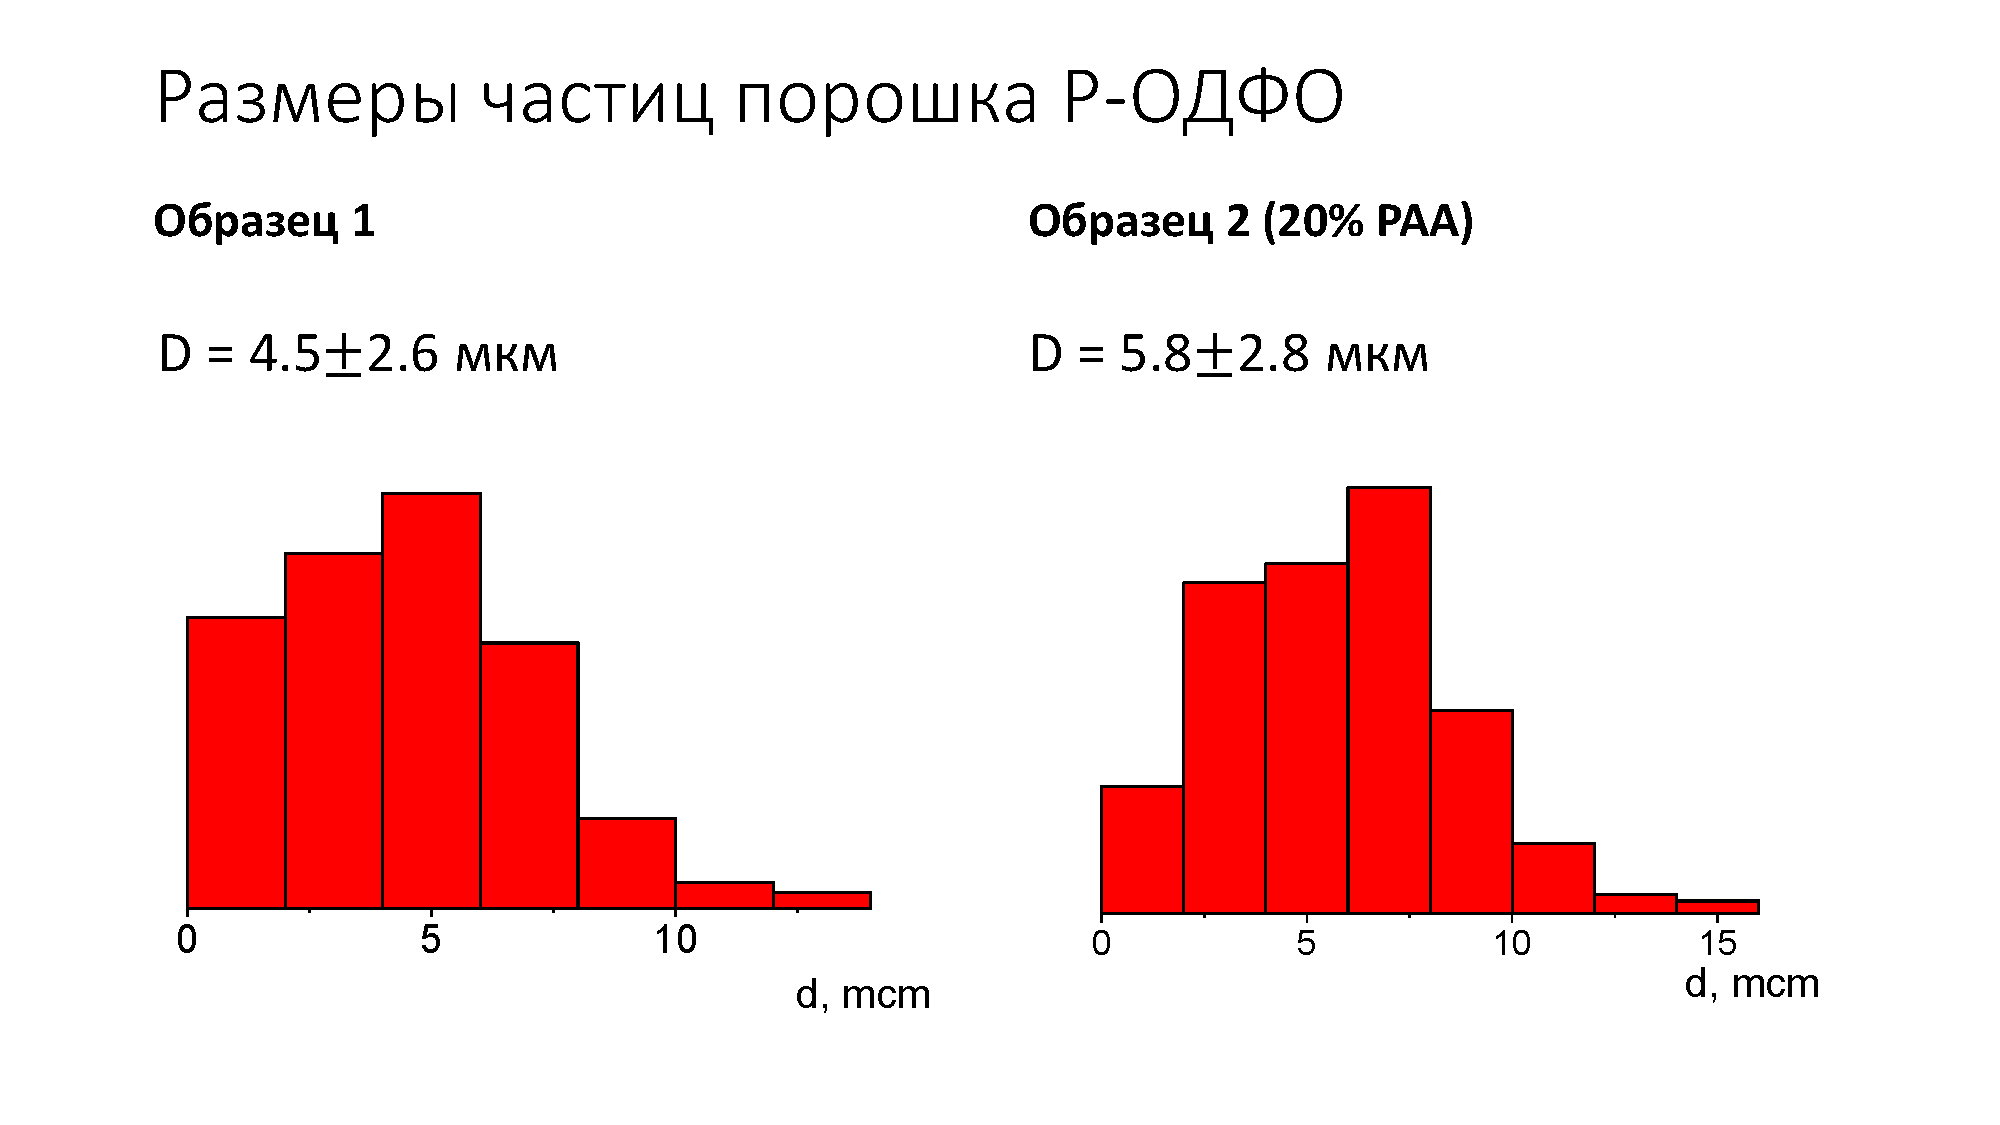
\includegraphics[width=\linewidth]{fig/particles}
	    \caption{Caption}
	    \label{fig:particles}
	\end{figure}
	
Измерения проводились на микрофокусной линии D13 Европейского центра синхротронного излучения (ERSF). Фото и схема ускоряющего кольца показаны на рис. \ref{fig:ring}. 
	
	
		\begin{figure}[h]\center
\begin{tabular}{cc}
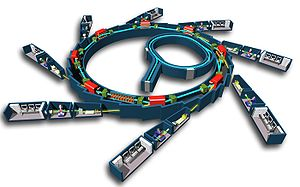
\includegraphics[width=0.5\linewidth]{fig/pribor-scheme.jpg}
&
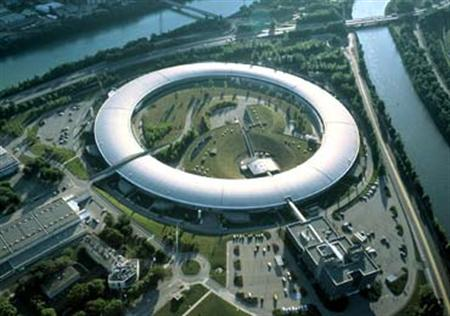
\includegraphics[width=0.5\linewidth]{fig/pribor-photo.jpg}
\end{tabular}
\caption{Синхротрон ERSF}
\label{fig:ring}
\end{figure}
	
А работает это так:
(тут еще картинка со схемой). Тогда получается большая интенсивность, бриллианс, статистика.



\section{[In progress]Схема эксперимента}
Общая схема
Принципиальная схемаизображена на рис. \ref{fig:experiment}. 

\subsection{Источник излучения}


\subsection{2D-детектор}

\subsection{Передвижение образца}


\begin{figure}[h]
    \centering
    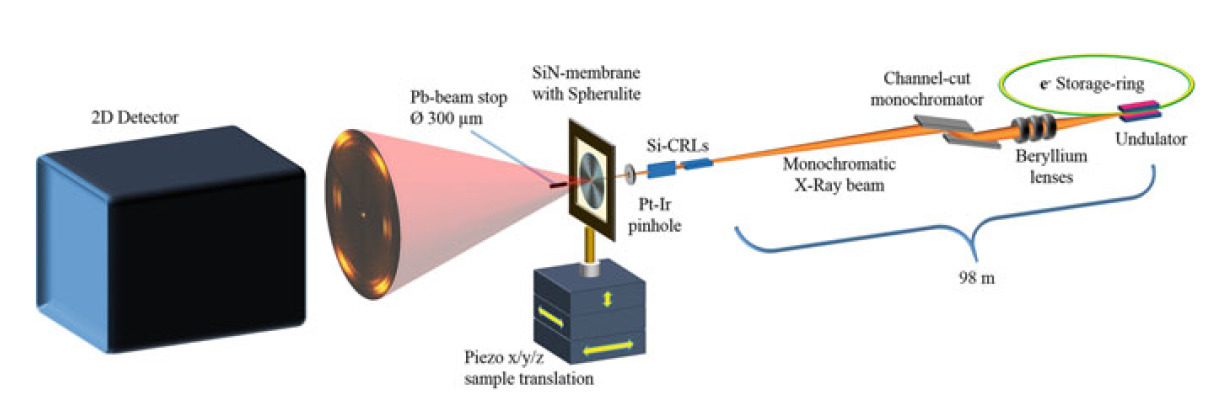
\includegraphics[width=\linewidth]{fig/ust.PNG}
    \caption{Экспериментальная установка. \cite{experiment}}
    \label{fig:experiment}
\end{figure}

\subsection{Калибровка}


 6.2.1 из 2д дифркции
 
 упомянуть про прочий подгон
 
Калибровка, а также азимутальное интегрирование производилось с помощью библиотеки pyFAI, \cite{pyfai}.



